\documentclass{article}
\usepackage{formatting}
\usepackage{multicol}
\usepackage{matlab-prettifier}

\title{Creating and Visualizing Curves and Surfaces: Answer Key}
\author{Quantitative Engineering Analysis}
\date{\today}

\begin{document}

\maketitle

\section{Sections}

\paragraph{1. Pick a fruit or vegetable, slice it in three ways, and sketch the sets of curves defined by each of these sets of slices.} 

You can choose whatever fruit/vegetable you want for this. Below is an example done with an eggplant, a great source of dietary fiber:

\begin{figure}[h!]
    \centering
    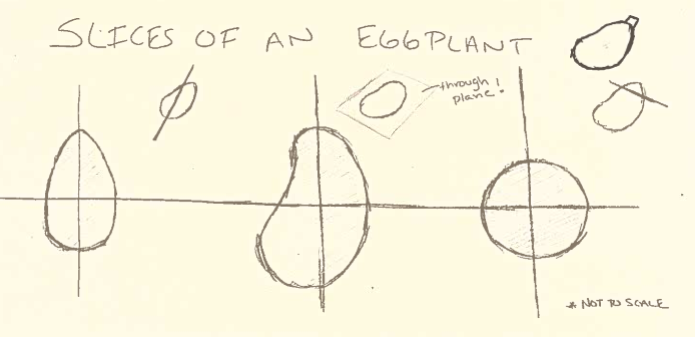
\includegraphics[width=0.55\columnwidth]{figs_and_code/slices_eggplant.jpg}
    \caption{Good `ol sketching.}
\end{figure}

\paragraph{2. Pick a manufactured object, imagine slicing it in three ways, and sketch the set of curves defined by each of these sets of slices.} 

Again, you can choose whatever you want for this. Below is an example done with a wine glass.

\begin{figure}[h!]
    \centering
    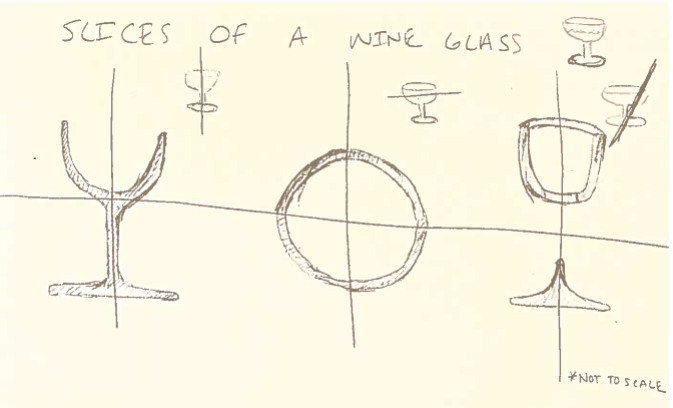
\includegraphics[width=0.55\columnwidth]{figs_and_code/slices_wine.jpg}
    \caption{Good `ol sketching.}
\end{figure}

\vspace{10cm}

\paragraph{3. Create a representation of one of these objects by cutting sections out of 1 inch blue foam and gluing them together.} 

Please provide a picture of your finished model. If you need help thinking about assembling something via sections, the photo below captures a bit about what we are talking about here:

\begin{figure}[h!]
    \centering
    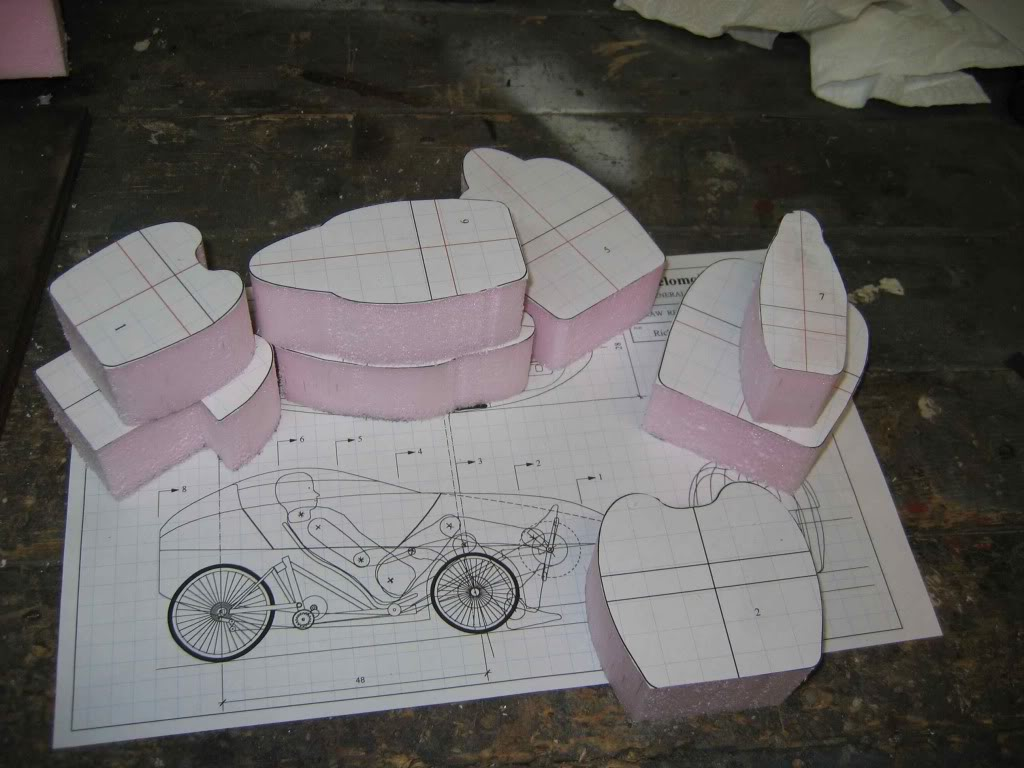
\includegraphics[width = 0.55\columnwidth]{figs_and_code/moremodelsections.jpg}
    \caption{An inspirative image of creating a model with layers.}
\end{figure}


\section{Symmetry}

\paragraph{4. Identify any reflection of rotation symmetries of your objects. Sketch your most symmetric object and indicate reflection planes and rotation axes of symmetry.} 

We decided to select our wine glass for this activity (perhaps for obvious reasons). What you provide should look similar to this:

\begin{figure}[h!]
    \centering
    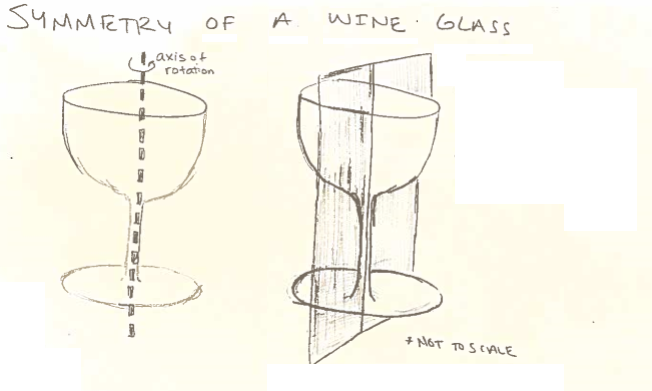
\includegraphics[width=0.75\columnwidth]{figs_and_code/symmetry_wine.png}
    \caption{An axis, and a plane. You'll notice that there are infinite symmetrical planes assuming that the rotation axis lies within the plane.}
\end{figure}

\section{Coordinates}

\paragraph{5. For both the fruit/vegetable and the manufactured object, propose two different origins and orientations of the coordinate system. What are the pros and cons of each one?} 

With our objects:

\begin{figure}[h!]
    \centering
    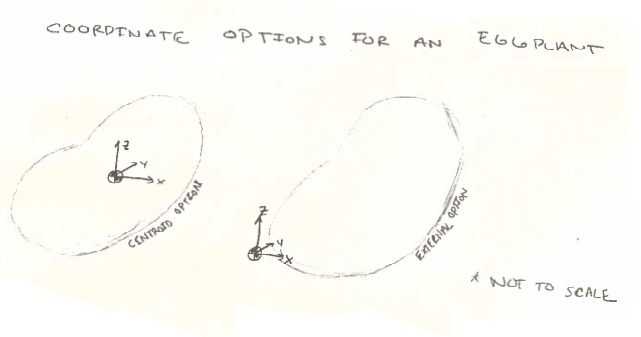
\includegraphics[width=0.55\columnwidth]{figs_and_code/coordinate_eggplant.jpg}
    \caption{Good `ol sketching.}
\end{figure}

\begin{figure}[h!]
    \centering
    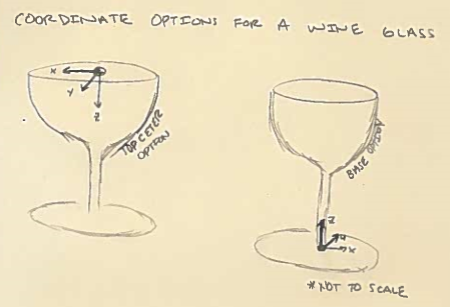
\includegraphics[width=0.55\columnwidth]{figs_and_code/coordinate_wine.jpg}
    \caption{Good `ol sketching.}
\end{figure}


\section{Curves Defined Explicitly by f = f(x)}

\paragraph{6. Compile a table of basic, explicit functions. Include their name, a sketch, and a function definition. Your  table should include polynomials, trigonometric functions, exponential, and logarithms.} 

You should make sure that you cover at least one each of: Linear, Polynomial, Exponential, Logarithmic, and Trigonometric function types. Basically, you should create a pretty typical ``parent function chart" similar to the one below. If you have more than that, wonderful!

\begin{figure} [h!]
    \centering
    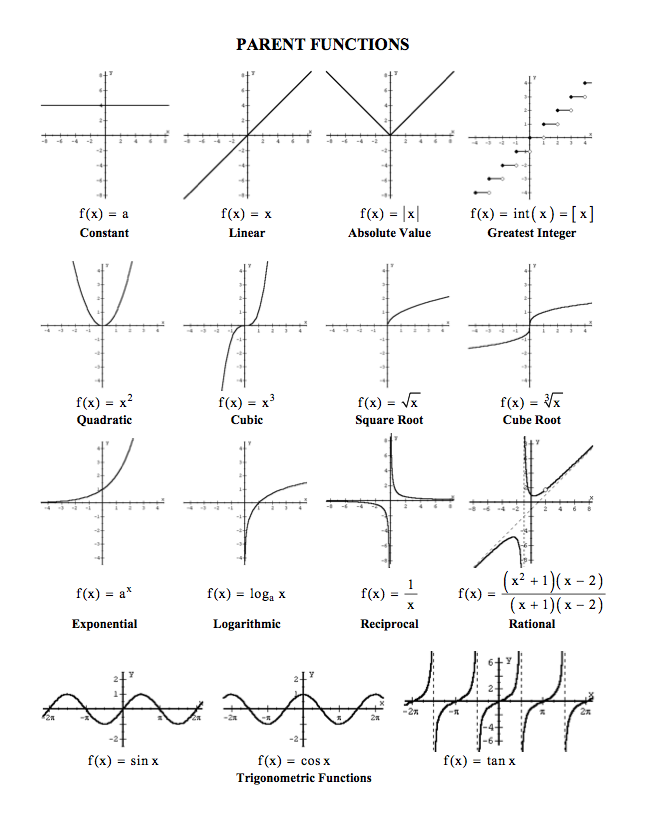
\includegraphics[width=1\columnwidth]{figs_and_code/parentfunctions.png}
    \caption{Remember these from middle/high school?}
\end{figure}

\vspace{5cm}

\paragraph{7. Choose a couple of curves that you sketched earlier (fruit, vegetable, object) and propose an explicit function that approximates some section of the curve. Using either Wolfram Alpha or MATLAB, check that your explicit function looks right.} 

Please have drawn your section of the curve next to a figure of the approximate explicit function, which you should identify. For our eggplant, we created a circle for the cross section. We have also included code and graphs of a parabola and a hyperbola graphed explicitly for your convenience.

\lstinputlisting[style=Matlab-editor,caption=code to plot explicit 2-d equations]{figs_and_code/explicit_2d.m}

\begin{figure}
    \centering
        \begin{minipage}{0.3\textwidth}
            \centering
            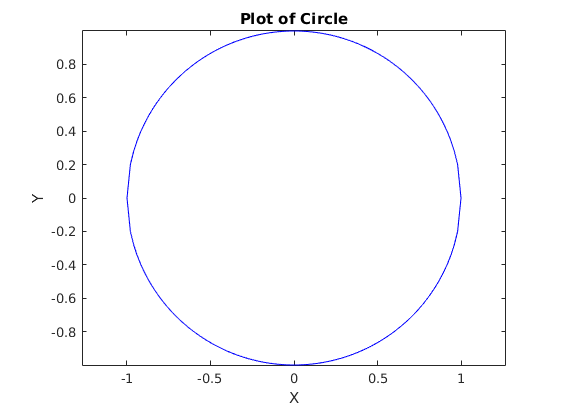
\includegraphics[width=\linewidth]{figs_and_code/circle.png}
            \caption{A circle.}
        \end{minipage}\hfill
        \begin{minipage}{0.3\textwidth}
            \centering
            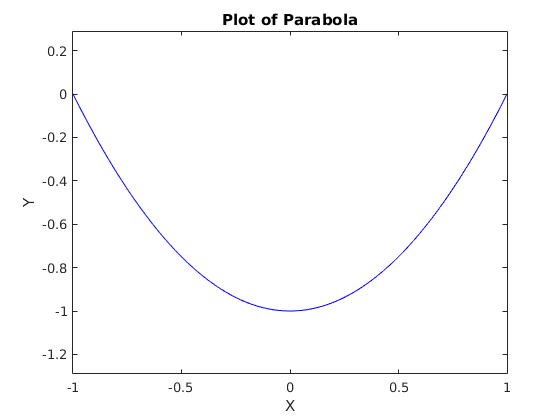
\includegraphics[width=\linewidth]{figs_and_code/parab.png}
            \caption{A parabola.}
        \end{minipage}\hfill
        \begin{minipage}{0.3\textwidth}
            \centering
            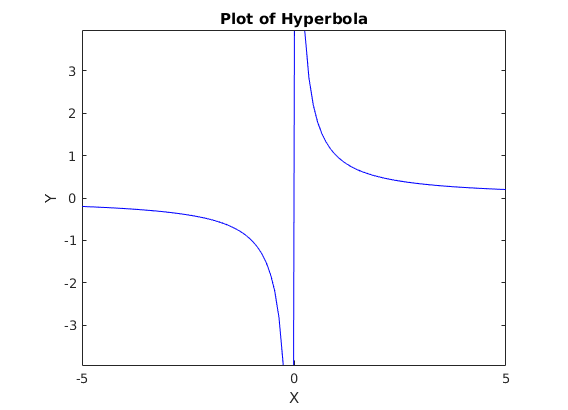
\includegraphics[width=\linewidth]{figs_and_code/hyperbola_2d.png}
            \caption{A hyperbola.}
        \end{minipage}\hfill
\end{figure}

\section{Curves Defined Implicitly by f(x,y)=0}

\paragraph{8. Review a catalogue of the conic sections. Pick out a couple of your favorites. Name them, sketch them, and write down the implicit function that defines them.} 

You can do what you want here, most of the Internet should be able to help you find the catalogue referenced: \url{http://paulbourke.net/geometry/conic/}. 

\begin{figure}[h!]
    \centering
    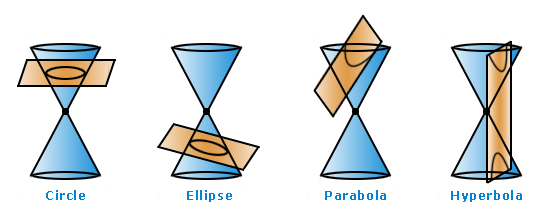
\includegraphics[width=0.75\columnwidth]{figs_and_code/conicsections.png}
    \caption{Conic sections illustrated with planes.}
\end{figure}

Circle: $x^2 + y^2 = r^2$, in which $r$ is the radius

Ellipse: $\dfrac{x}{a}^2 + \dfrac{y}{b}^2 = 1$, in which $a$ and $b$ are the radius on the x and y axis, respectively. 

Parabola: $4ax = y^2$, in which $a$ is the focus of the curve. 

Hyperbola: $\dfrac{x}{a}^2 - \dfrac{y}{b}^2 = 1$, in which $a$ and $b$ are the foci of the curves.


\paragraph{9. Would any of your curves from earlier be better represented with an implicit function? If so, propose one.} 

We realize that most fruits/vegetables will probably be used here (depending on how ``organic" your manufactured object is). For our eggplant, we think that a circle or an ellipse will probably fit the bill for some of our curves and be better approximations than perhaps an explicit function.

\paragraph{10. If you propose an implicit function to represent one of your curves, visualize that function using the computational tool of your choice. If you did not propose an implicit function, visualize the curve $f(x,y) = x^2 + xy + y^2 - 1 - y - 1 = 0$.} 

Be sure to document which visualization you created. Below we generated a graph of the implicit curve provided using \texttt{ezplot}:

\lstinputlisting[style=Matlab-editor,caption=code to plot implicit 2-d equations]{figs_and_code/implicit_2d.m}

\begin{figure} [h!]
    \centering
    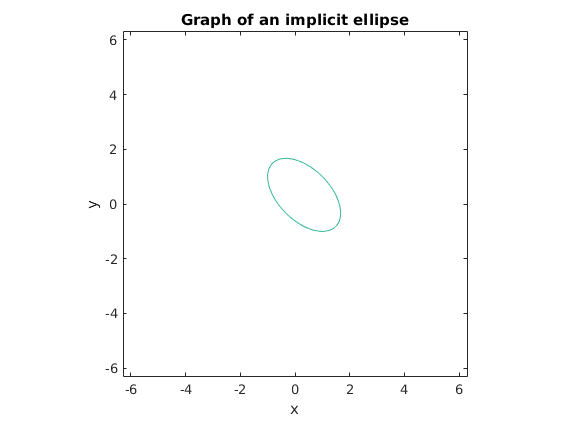
\includegraphics[width=1\columnwidth]{figs_and_code/ellipse.png}
    \caption{We love you \texttt{ezplot}!}
\end{figure}

%%%%%%%%%%%%%%%%%INSERT VISUALIZATIONS%%%%%%%%%%%%%%%%%% %NEED TO DO. PLEASE PROVIDE THE MATLAB CODE WHICH CREATED THIS VISUALIZATION

\section{Surfaces Defined Explicitly by z=f(x,y)}

This section didn't have any specific questions. If you have any, please talk to an instructor or NINJA! If you want an example of how to plot an explicit 3-d function in MATLAB, here you go!

\lstinputlisting[style=Matlab-editor,caption=code to plot explicit 3-d equations]{figs_and_code/explicit_3d.m}

\begin{figure} [h!]
    \centering
        \begin{minipage}{0.3\textwidth}
            \centering
            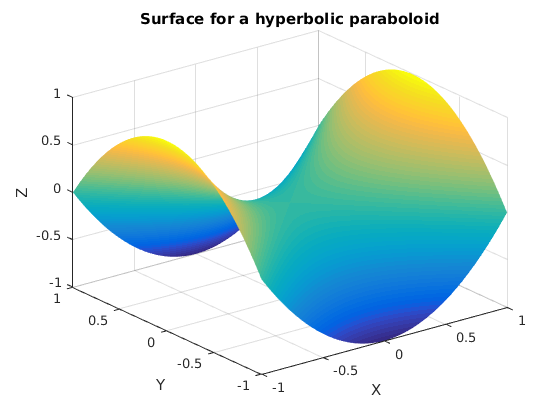
\includegraphics[width=\linewidth]{figs_and_code/hyp_parab_3d.png}
        \end{minipage}\hfill
        \begin{minipage}{0.3\textwidth}
            \centering
            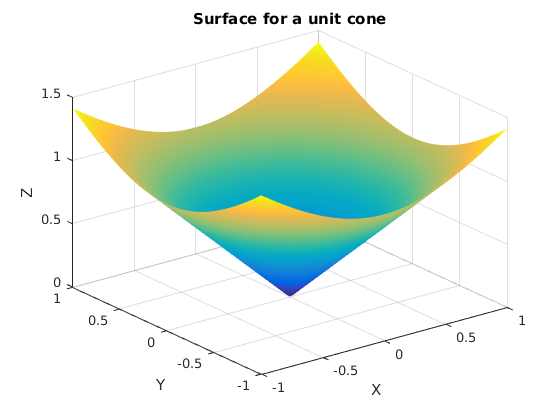
\includegraphics[width=\linewidth]{figs_and_code/cone_3d.png}
        \end{minipage}\hfill
        \begin{minipage}{0.3\textwidth}
            \centering
            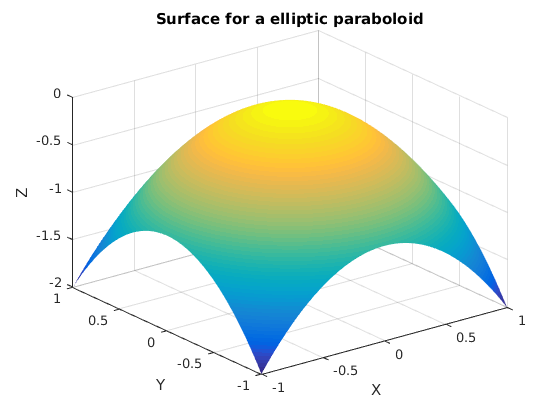
\includegraphics[width=\linewidth]{figs_and_code/elip_parab_3d.png}
        \end{minipage}\hfill
\end{figure}

\section{Surfaces Defined Implicitly by f(x,y,z)=0}

\paragraph{11. Review a catalogue of the quadric surfaces. Pick out a couple of your favorites. Name them, sketch them, and write down the function that defines them.} 

Just like in the conic problem, this can be handled with the aid of the Internet: \url{http://www.math.tamu.edu/~kahlig/notes/251/12-6-table-01.gif}. 

\begin{figure}[h!]
    \centering
    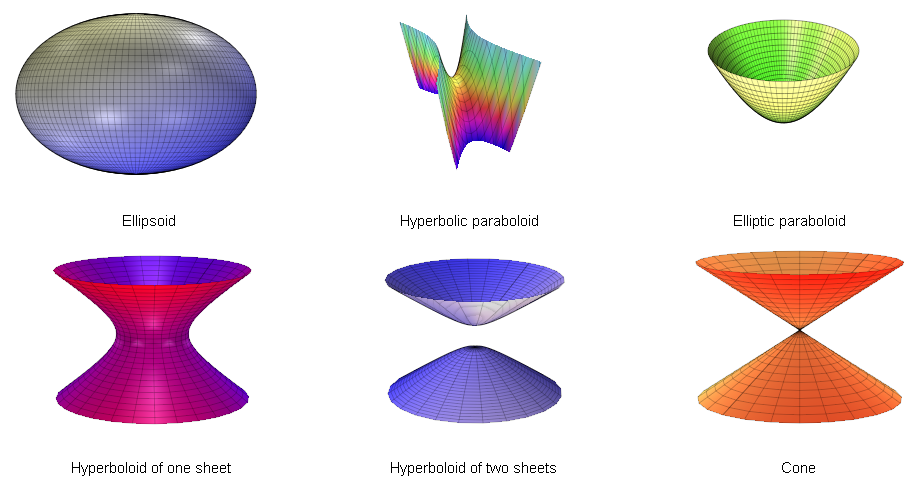
\includegraphics[width=0.65\columnwidth]{figs_and_code/quadric.png}
    \caption{A quadric/quadratic surface chart. Pretty groovy right?}
    
\end{figure}

Ellipsoid: $\dfrac{x}{a}^2 + \dfrac{y}{b}^2 + \dfrac{z}{c^2} = 1$

Elliptic Paraboloid: $\dfrac{x}{a}^2 + \dfrac{y}{b}^2 = \dfrac{z}{c}$

Hyperbolic Paraboloid: $\dfrac{x}{a}^2 - \dfrac{y}{b}^2 = \dfrac{z}{c}$

Cone: $\dfrac{x}{a}^2 + \dfrac{y}{b}^2 = \dfrac{z}{c}^2$

Hyperboloid. 1 Sheet: $\dfrac{x}{a}^2 + \dfrac{y}{b}^2 - \dfrac{z}{c}^2 = 1$

Hyperboloid, 2 Sheets: $-\dfrac{x}{a}^2 - \dfrac{y}{b}^2 + \dfrac{z}{c}^2 = 1$ 


\paragraph{12. Choose a fruit/vegetable or manufactured object and propose an explicit or implicit representation of its surface.} 

You can do whatever you want here, but we hope you thought about more complicated objects than baseballs, basketballs, golf balls...One interesting example would be to use a hyperboloid of one sheet to model a stool or other form of seating. Perhaps an elliptic paraboloid could become that wine glass we talked about earlier. 

\paragraph{13. Visualize your chosen representation using an appropriate computational tool.}

The NINJAs were able to find two different ways of plotting implicit 3-d surfaces in matlab. The first is to define the functions parametrically and using \texttt{ezsurf}. The other is a bit more complicated code wise, but easier math-wise, as you don't need to any separate algebra. The other way involves using the \texttt{isosurface}. We've demonstrated both below:

\lstinputlisting[style=Matlab-editor,caption=code to plot implicit 3-d equations parametrically. Note that we had to derive the equation for a hyperboloid of one sheet before writing this code.]{figs_and_code/implicit_3d_parametric.m}

\begin{figure}[h!]
    \centering
    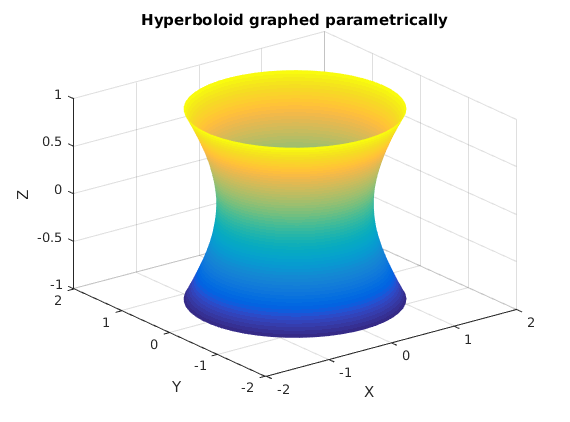
\includegraphics[width=0.65\columnwidth]{figs_and_code/hyperboloid_1_parametric.png}
    \caption{Wow such paraboloid!}
\end{figure}

\lstinputlisting[style=Matlab-editor,caption=code to plot implicit 3-d equations using \texttt{isosurface}.]{figs_and_code/implicit_3d.m}

\begin{figure} [h!]
    \centering
        \begin{minipage}{0.3\textwidth}
            \centering
            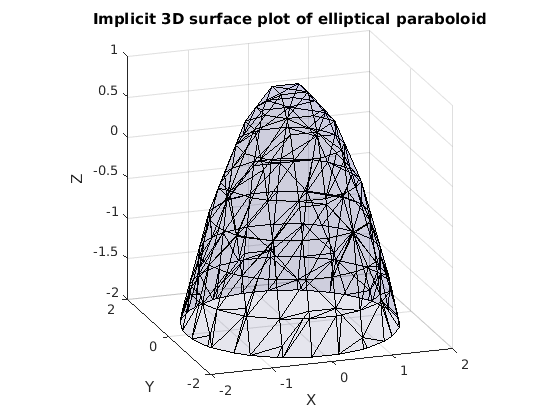
\includegraphics[width=\linewidth]{elip_parab_3d_implicit.png}
        \end{minipage}\hfill
        \begin{minipage}{0.3\textwidth}
            \centering
            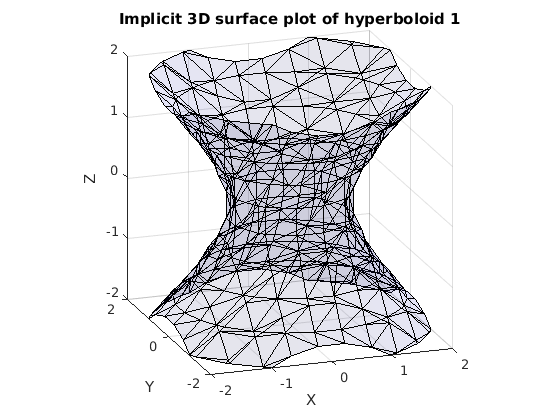
\includegraphics[width=\linewidth]{hyperboloid_1_implicit.png}
        \end{minipage}\hfill
        \begin{minipage}{0.3\textwidth}
            \centering
            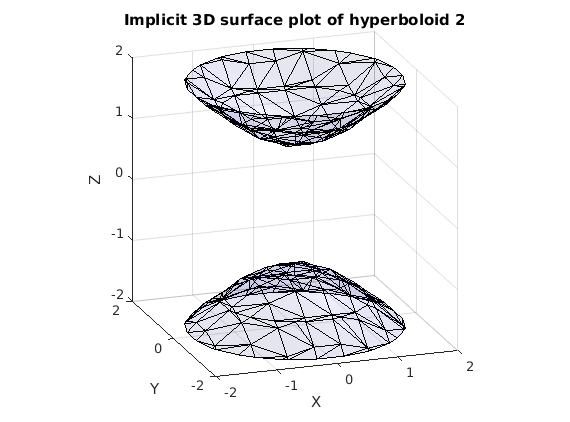
\includegraphics[width=\linewidth]{hyperboloid_2_implicit.png}
        \end{minipage}\hfill
\end{figure}

\section{Surfaces Defined by Sweeping}

\paragraph{14. Create approximate surfaces of the fruit/vegetable and manufactured object by using the Sweeping tool in Solidworks. Discuss the ways in which the approximate surfaces fails to match that of the object. If it matches the surface of the object, then please explain why.} 

You could use your original things or your new thing that you used in the previous problem. It doesn't really matter. Below, we try to create sweeps of our wineglass. We were pretty successful in using our sweep by making our guide curve the outer glass profile, then drafting a circle along the curve.

\begin{figure}[h!]
    \centering
    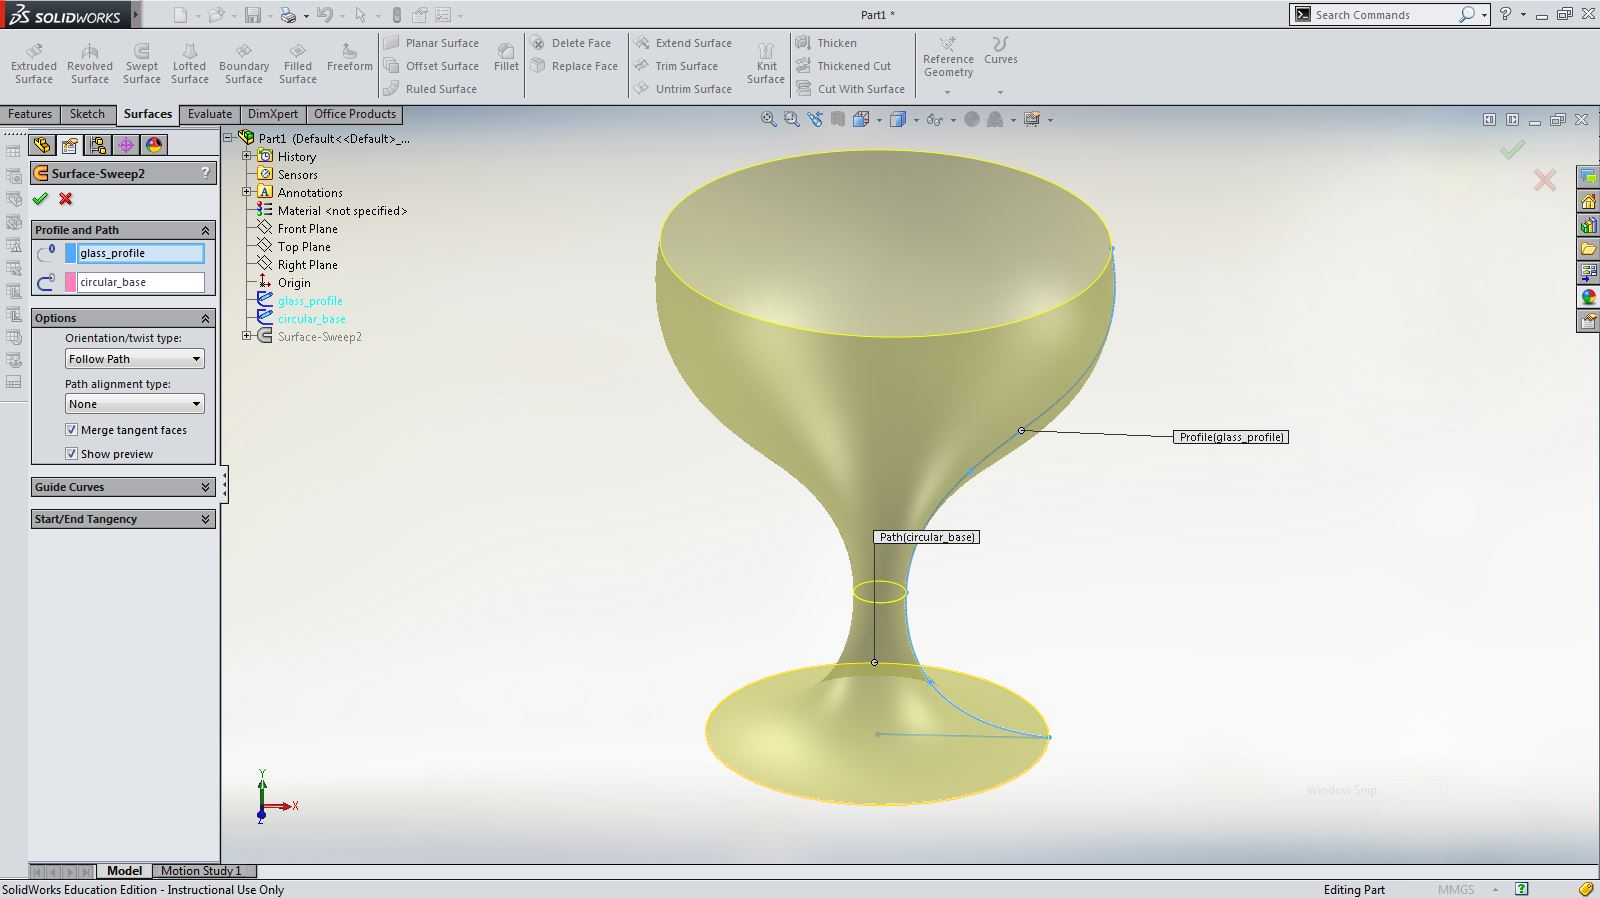
\includegraphics[width=1\textwidth]{figs_and_code/QEA_sweep}
    \caption{Surface sweeping}
\end{figure}

\section{Surfaces Defined by Revolution}

\paragraph{15. Record and sketch at least five objects (natural or manufactured) which have a surface of revolution or part of one. Identify at least one axis of motion.} 

You can do whatever you want here, please draw a sketch and label the axes you identify. Some objects we thought were interesting are below:

\begin{itemize}
    \item egg
    \item dining hall salt shaker
    \item water bottle
    \item car tire
    \item sailboat mast
\end{itemize}

\paragraph{16. Choose one of them and sketch the boundary curve obtained by making an imaginary cut along a plane containing the axis of rotation.}

Your should be looking to have a ``half" outline of one of your shapes in order to do this. For an egg, that may look like a simple curve which meets the axis of rotation. For a car tire, that might be a circle that is some distance away from the axis of rotation. 

\paragraph{17. Create an explicit function that approximates the boundary curve, and write down the equation that defines the surface of revolution.}

For our water bottle, which we'll abstract to a simple cylinder, we want to revolve a line (we'll call our line y = 3) about the x-axis. Using the form of the equation found in the Pset, that means our explicit function for the curve is $f(x) = 3$ and our surface could then be described implicitly as $y^2 + z^2 = 9$.

For our lovely wineglass, we may define that profile as something like $f(x) = sin(x)$ (yes we realize this is extremely simplistic). The surface would in this case would be described as $y^2 + z^2 = sin^2(x)$.

\paragraph{18. Create this surface in Solidworks.} 

First you need an axis to revolve the profile around:
\begin{figure}[h!]
    \centering
    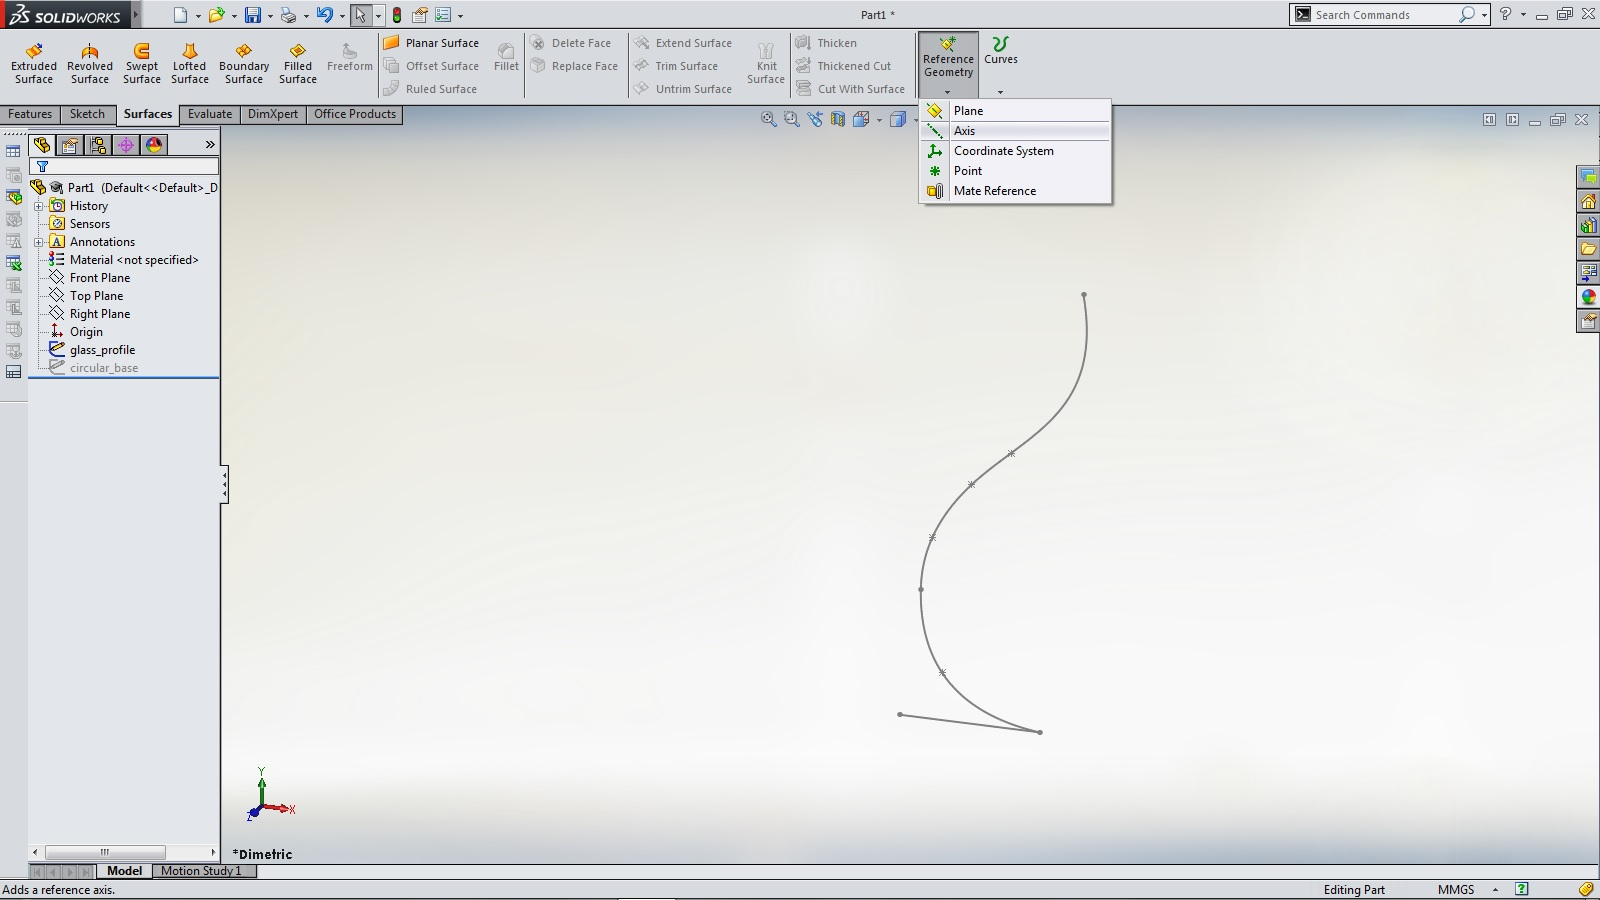
\includegraphics[width=1\textwidth]{figs_and_code/QEA_axis1}
    \caption{Creating an axis to revolve around}
\end{figure}

\begin{figure}[h!]
    \centering
    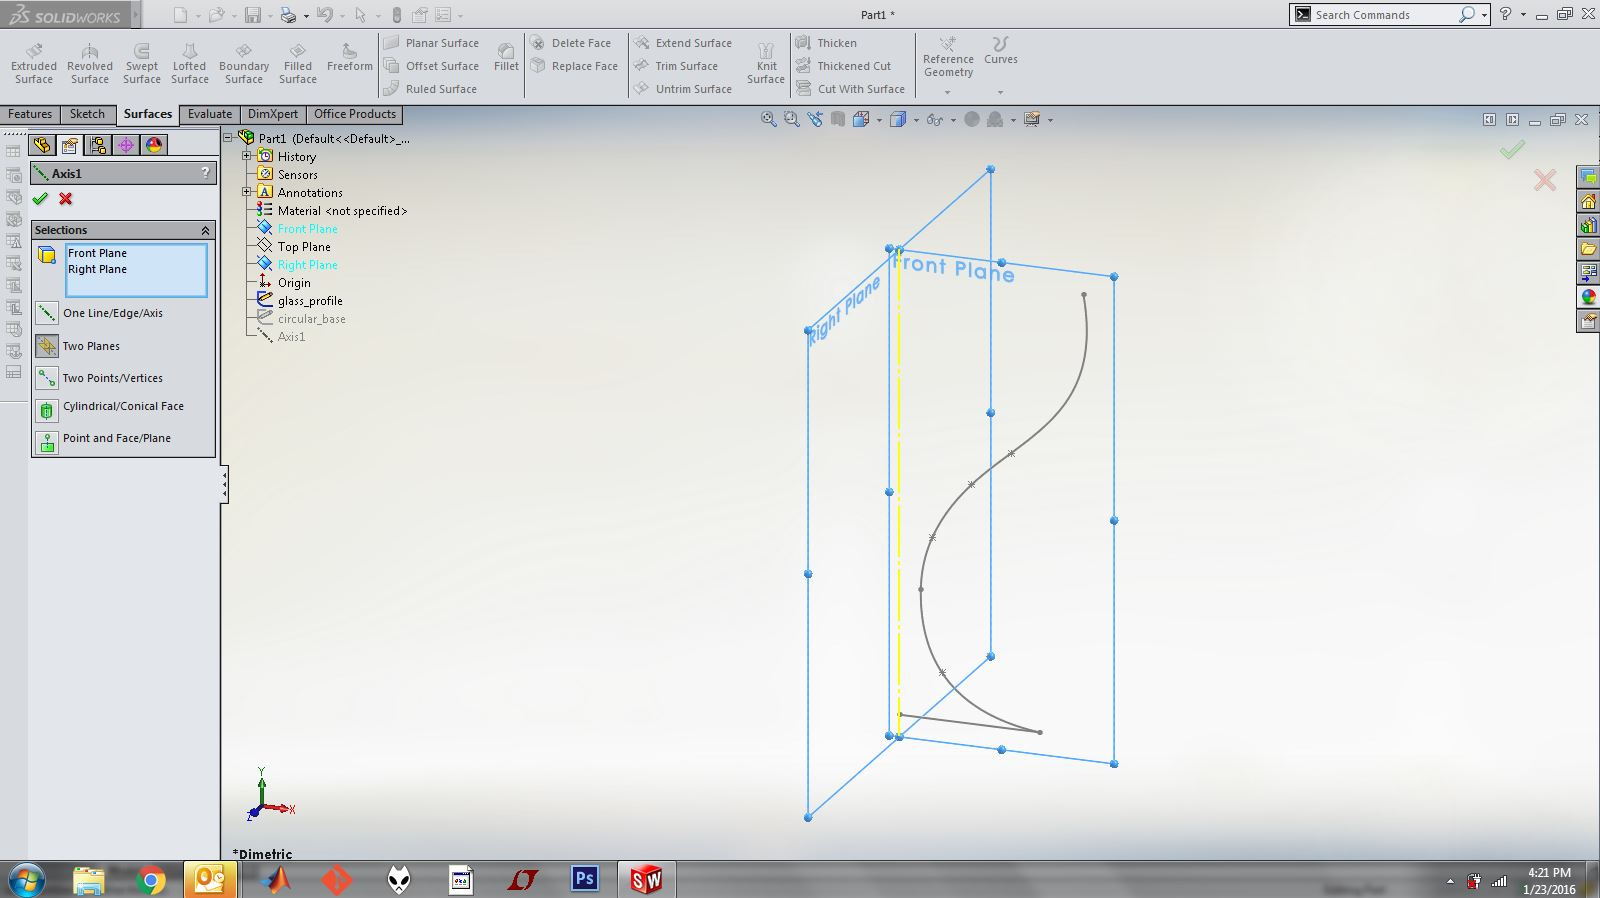
\includegraphics[width=1\textwidth]{figs_and_code/QEA_axis2}
    \caption{Creating an axis to revolve around}
\end{figure}

Then you can revolve the profile around the axis:

\begin{figure}[h!]
    \centering
    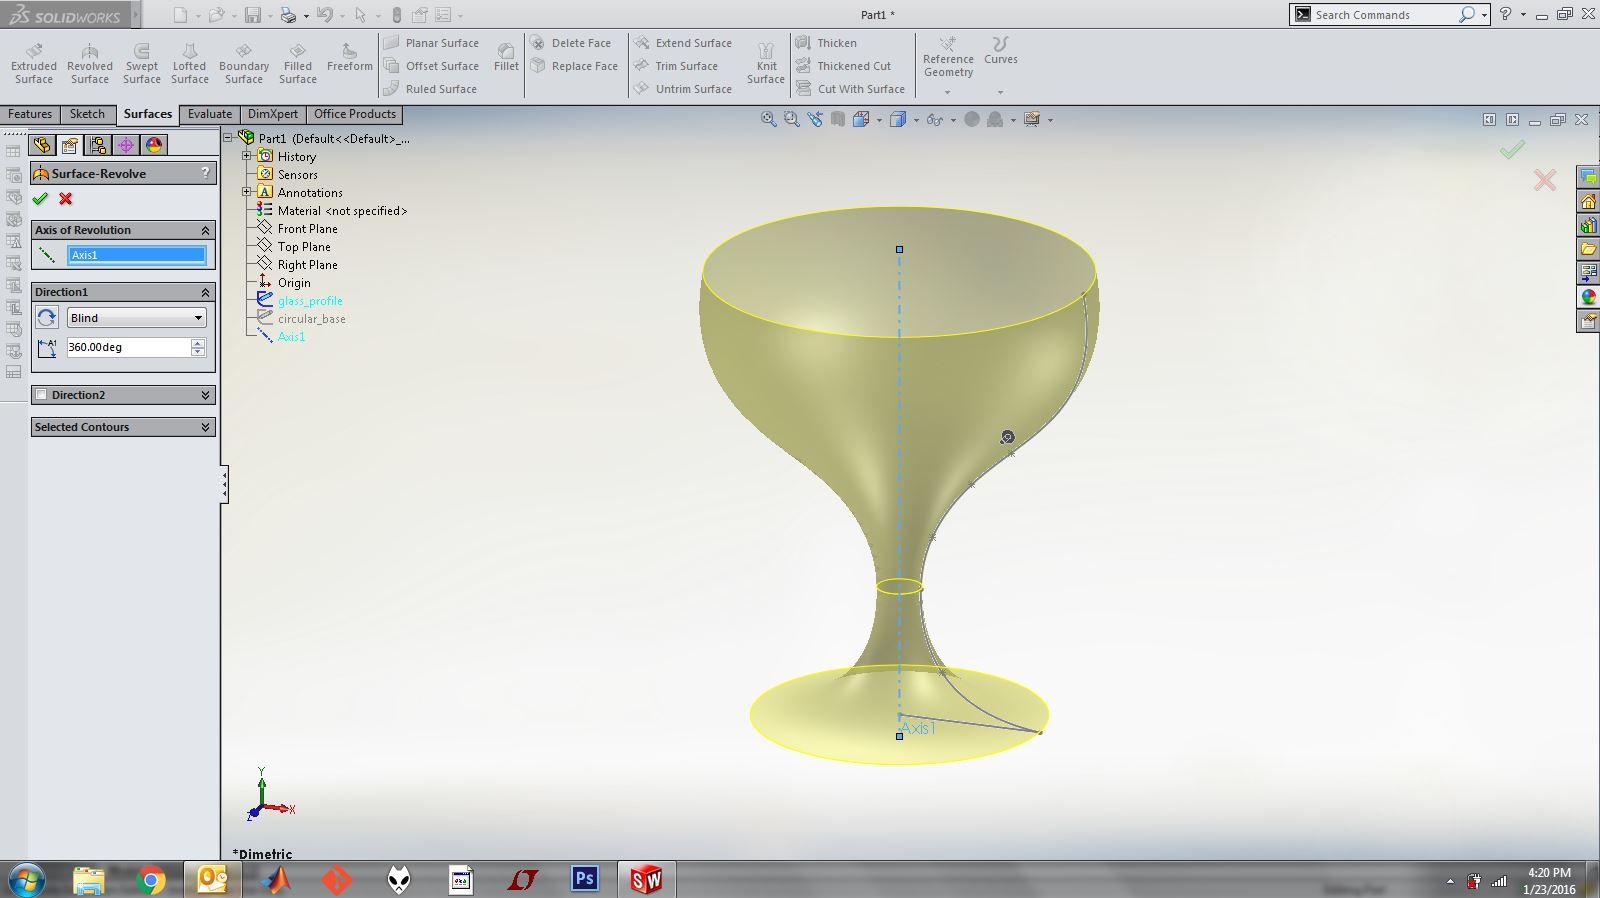
\includegraphics[width=1\textwidth]{figs_and_code/QEA_revolve}
    \caption{revolve the profile around the axis}
\end{figure}

%%%%%%%%%%%%%%% INSERT EXAMPLE %%%%%%%%%%%%% %NEED TO DO THIS

\section{Surfaces Defined by Lofting}

\paragraph{19. Choose a fruit, vegetable, or manufactured object, and create an approximation to the surface by lofting.}

For our wineglass, we could use three lofting points at the base, stem, and rim to loft between. We'll start from the base and go to the stem to illustrate this process. $f_1(x) = \sqrt{x^2 - 2^2}$ and $f_2(x) = \sqrt{x^2 - 1^2}$ roughly match these points, at (let's just arbitrarily say) $z = 0$ and $z = 2$. This means our lofted surface will be defined exactly like in the pset, and the shape we would get will kind look like a cone without the point. When we do the other side, this will look like an upside down cone...you get the picture. 

We could have also chosen to loft from base but (given the simplified equation you've been presented) that would look roughly like an upside down cone. In Solidworks, you can loft two curves along a given guide curve, which we illustrate in the next problem. What this does is take infinitesimally small points along the curve, extrapolates a surface at that point, and then lofts between the bottom surface and the extrapolated surface. This can yield some interesting results.


\paragraph{20. Create this surface in Solidworks.} 

First you need to create the beginning and end profiles of your loft. For a wine glass, these are just circles to indicate the base and lip of the glass. To create the lip circle, I needed to define a new plane to sketch the lip on:

\begin{figure}[h!]
    \centering
    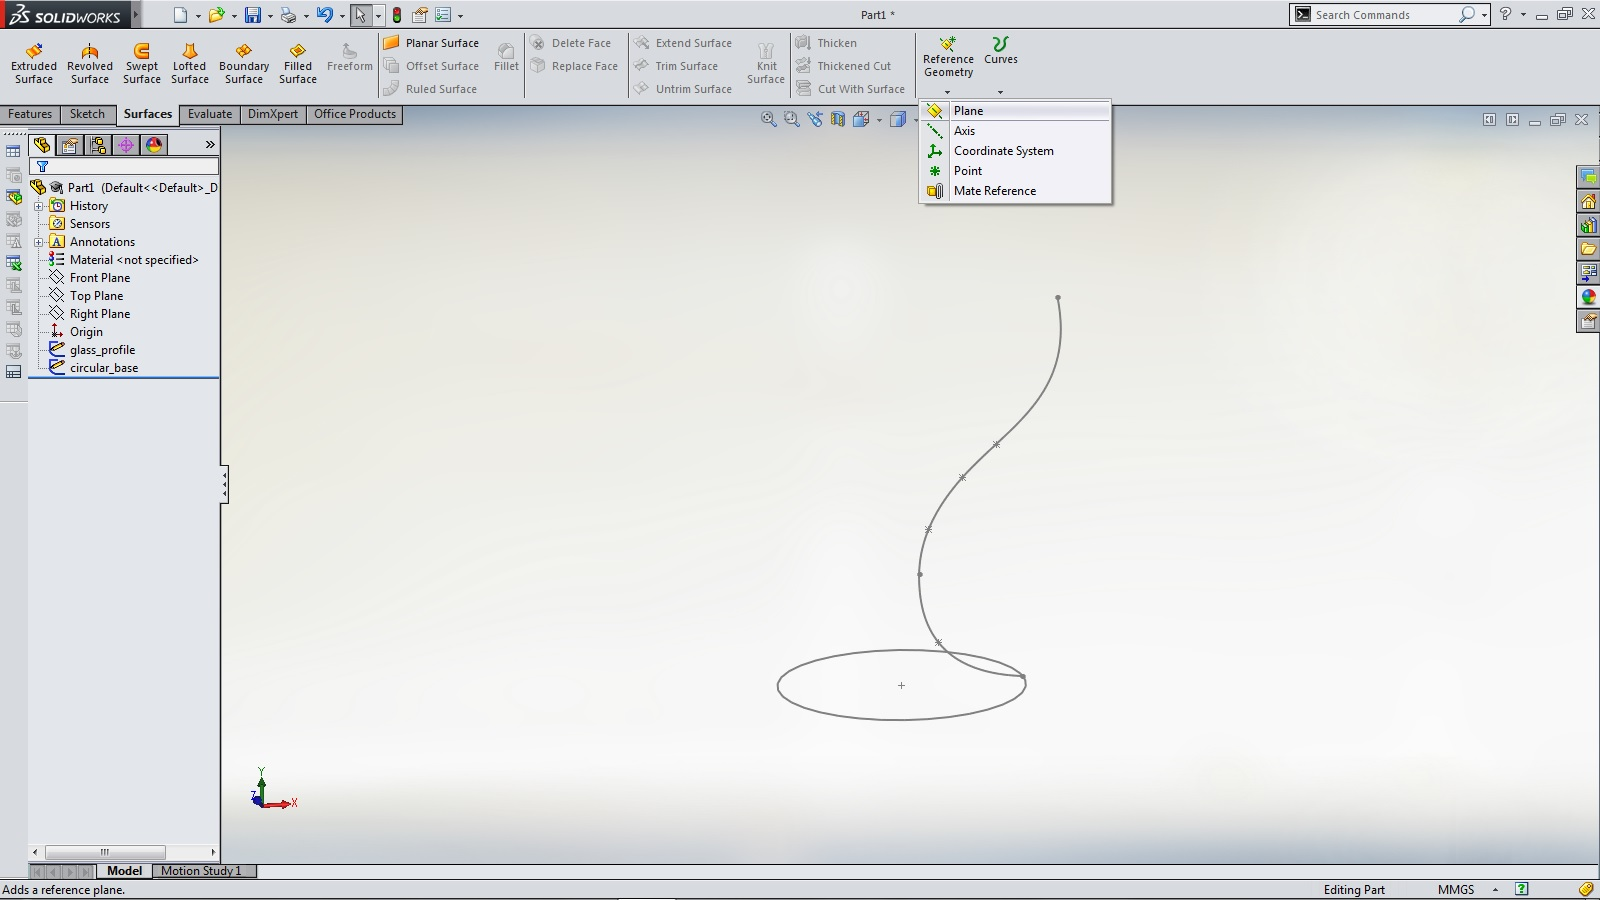
\includegraphics[width=1\textwidth]{figs_and_code/QEA_plane1}
    \caption{Creating a new plane}
\end{figure}

\begin{figure}[h!]
    \centering
    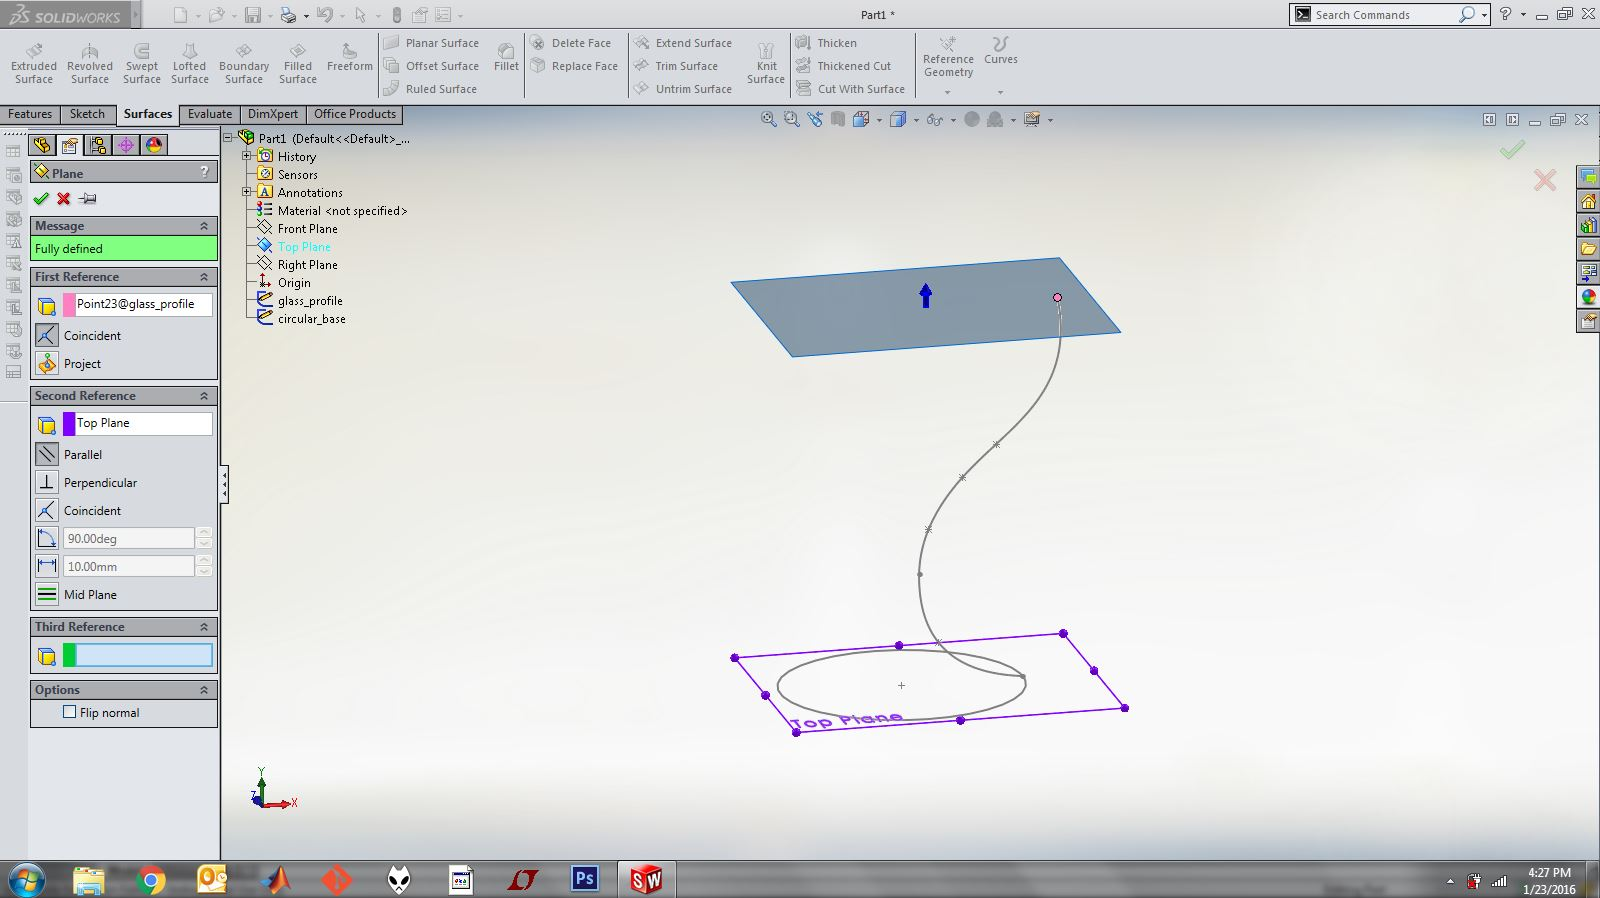
\includegraphics[width=1\textwidth]{figs_and_code/QEA_plane2}
    \caption{Creating a new plane}
\end{figure}

\begin{figure}[h!]
    \centering
    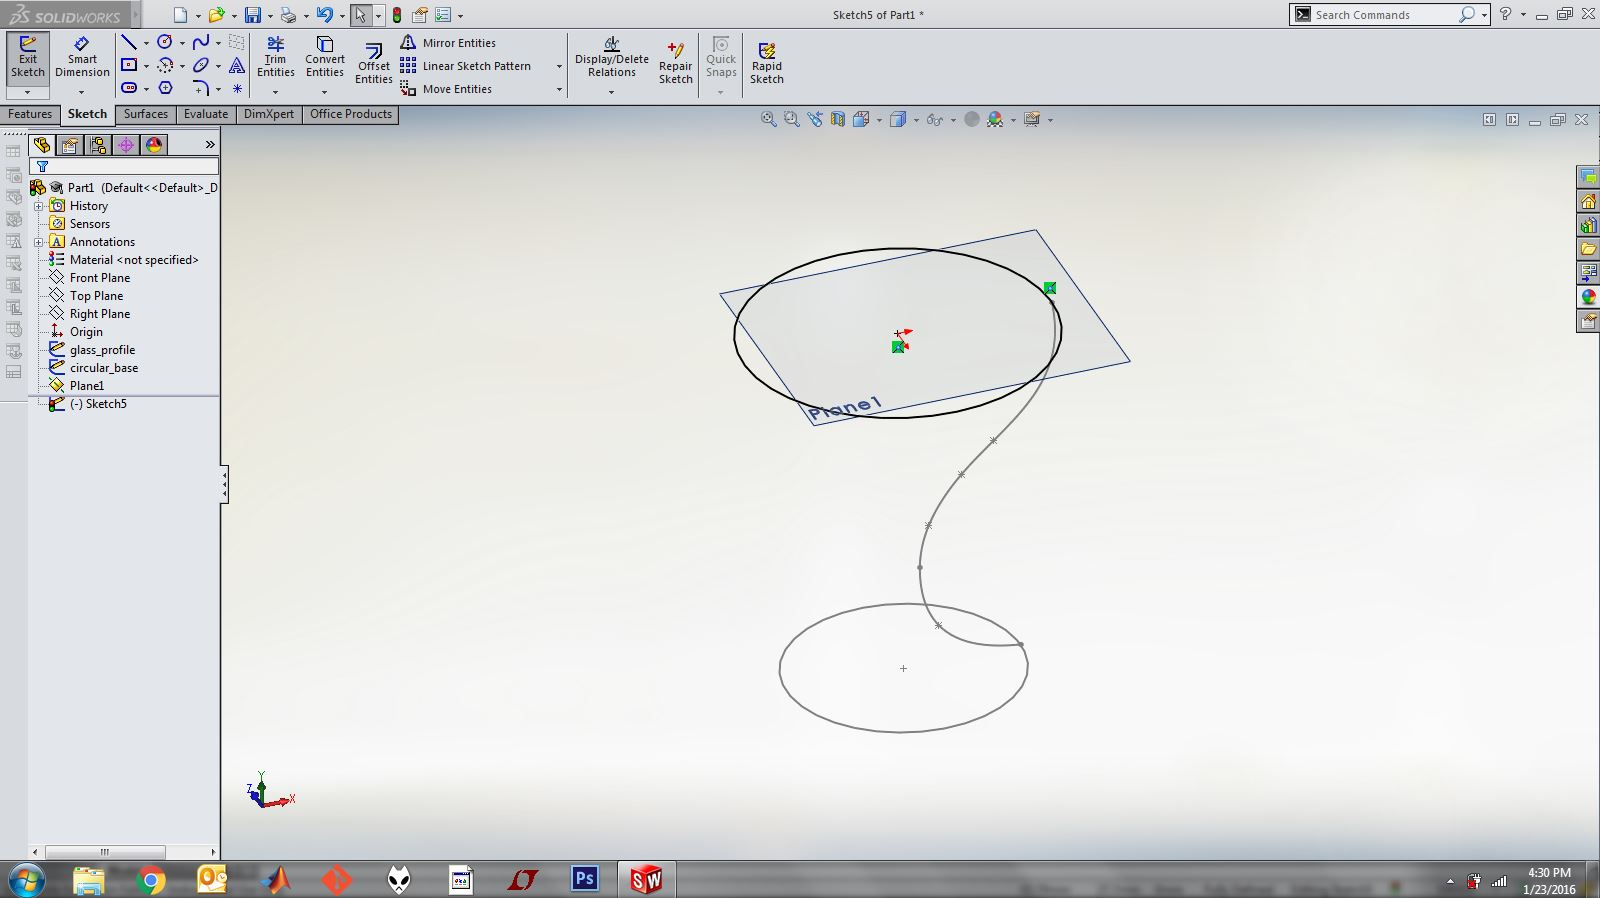
\includegraphics[width=1\textwidth]{figs_and_code/QEA_secondCircle}
    \caption{Now I can sketch the lip circle on the plane I created}
\end{figure}

\begin{figure}[h!]
    \centering
    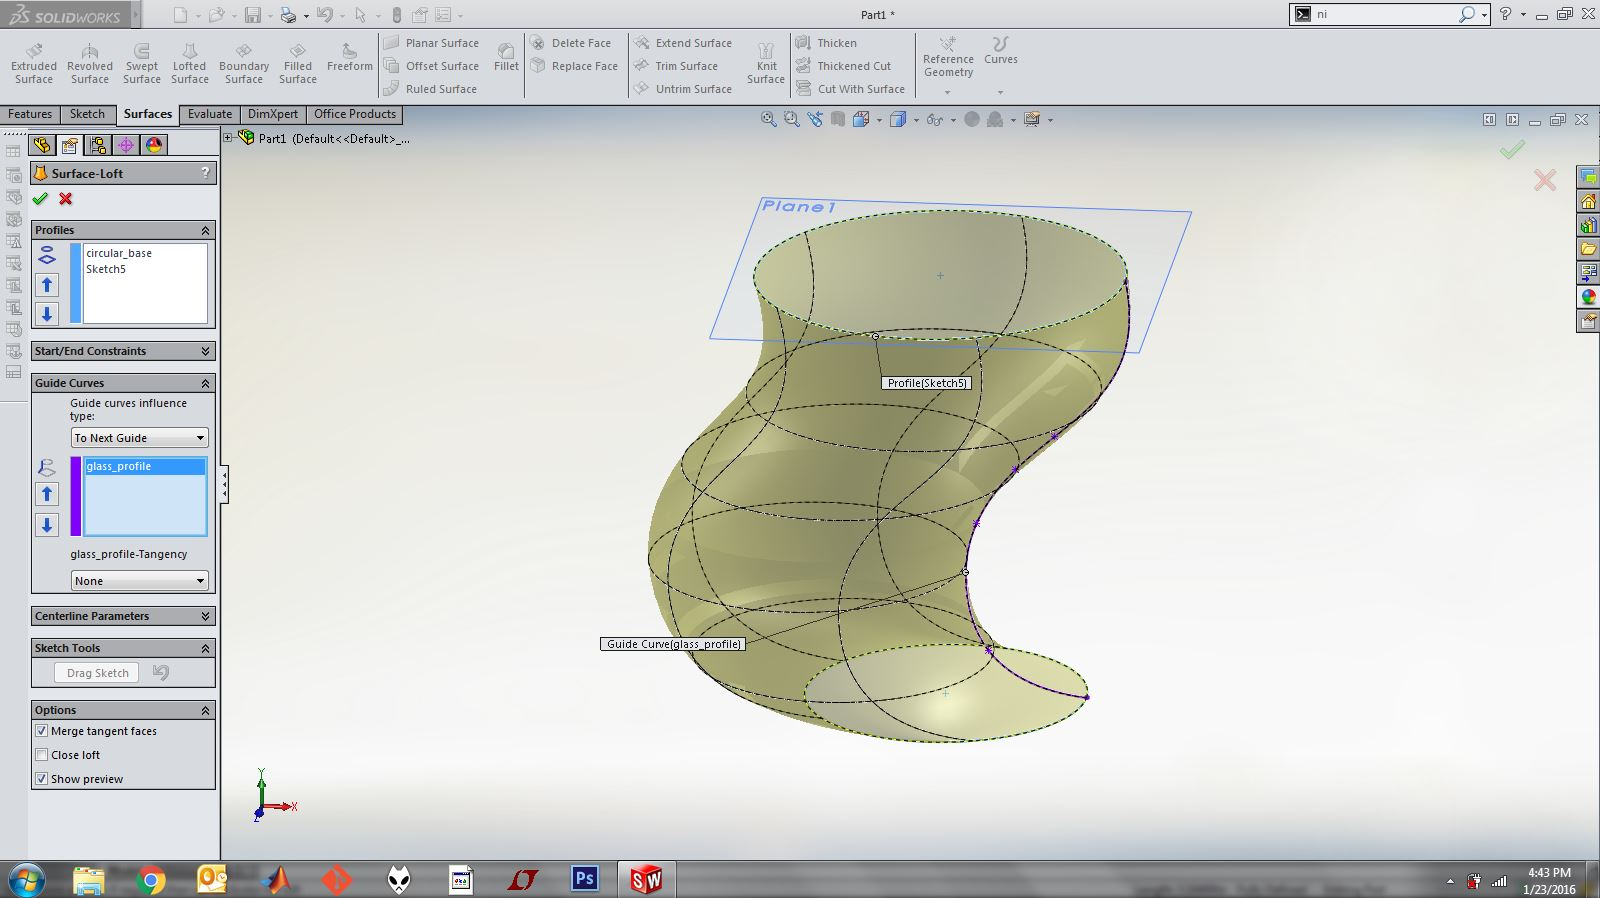
\includegraphics[width=1\textwidth]{figs_and_code/QEA_lofting}
    \caption{the final loft}
\end{figure}

Clearly this is no good. A loft is not well suited for our need.

A note about lofting, courtesy of Ariana and Eric: just as we explained above how Solidworks makes its loft, it is also critical that you be aware that the points along the lofting curve are also divided into an ``infinite" number of points which are associated with points on the curve it is being lofted to. This means that if these curves are "rotated" relative to each other, this may cause a twist in your loft. Imagine two equally sized circles, one on top of the other, being lofted. You might imagine a cylinder (in all of its cylinder glory). However, if (for some reason) Solidworks decides to associate the 6 o'clock point on the bottom circle to the 6:15 point on the top circle, you'll get a slightly hour glass shape. To prevent this from happening, you can associate your geometries more precisely with a variety of constraint/mate tools in Solidworks. 








\end{document}
